\section{Theorie}

\subsection{Ideale und reale Operationsverst{\"a}rker}
Ein Operationsverstärker ist ein gleichstromgekoppelter Differenzverstärker. Die Spannung am Ausgang $U_A$ entspricht der Differenz der Eingangsspannungen $U_P$ (am nicht invertierenden Eingang)
sowie $U_N$ (am invertierenden Eingang), die um den Verstärkungsfaktor $V$ verstärkt wird.
\begin{equation}
U_A = V (U_P - U_N)
\end{equation}
Das Schaltbild mit den entsprechenden Anschlüssen ist in \ref{abb:op} abgebildet.
\begin{figure}
 	\centering
 	\includegraphics[width=\textwidth]{img/op.png}
 	\caption{Schaltbild eines Operationsverstärkers}
 	\label{abb:op}
\end{figure}
Die Ausgangsspannung des Operationsverstärkers kann im Bereich der Betriebsspannungen varrieren:
\begin{equation}
-U_B < U_A < U_B
\end{equation}
Sollte $U_A$ außerhalb des von den Betriebsspannungen definierten Bereich leigen, so nimmt die Ausgangspannung den nächstliegenden Wert, also $-U_B$ oder $U_B$ an.

Um den Umgang mit realen Operationsverstärkern bei Berechnungen und in Schaltungen zu vereinfachen, wird das Modell des idealen Operationsverstärkers eingeführt:
Der ideale Operationsverstärker zeichnet sich durch eine unendlich große Leerlaufverstärkung, einem unendlichen Eigangswiderstand, sowie einem verschwindenen Eingangswiderstand aus.

Für reale Operationsverstärker gibt es weitere Eigenschaften, die erläutert werden müssen:
Sollte an beiden Eingängen die gleiche Spannung $U_G$ anliegen, müsste theoretisch $U_A = 0$ sein. Jedoch beobachtet man auf Grund der Unsymmetrien der beiden Kanäle eine Ausgangsspannung.
Der Quotient aus $U_G$ und $U_A$ wird Gleichtacktverstärkung
\begin{equation}
V_G = \frac{\delta U_A}{\delta U_G}
\end{equation}
genannt und ist ein Maß für die Abweichung vom idealen Operationsverstärker.
Ferner gibt es Eingangsströme auf Grund der endlichen Eingangswiderstände. Somit ist es möglich den Eingangsruhestrom
\begin{equation}
I_B = \frac{1}{2} (I_P + I_N)
\end{equation}
aus den Eingangsströmen $I_P$ (nicht invertierter Eingang) und $I_N$ (invertierter Eingang) zu berechnen.

Außerdem lässt sich der Offsetstrom definieren
\begin{equation}
I_0 = I_P - I_N.
\end{equation}
Aus den definierten Größen lässt sich der Differenzeingangswiderstand $r_D$ definieren:
\begin{equation}
r_D = \left\{\begin{array}{ll} \frac{\delta U_P}{\delta I_P}, für U_N = 0\\
	  \frac{\delta U_N}{\delta I_N}, für U_P = 0\end{array}\right\}.
\end{equation}
Auch ist für $U_G = U_P = U_N$ und $I_G = I_P + I_N$ der Gleichtakteingangswiderstand
\begin{equation}
r_G = \frac{\delta U_G}{\delta I_G}
\end{equation}

\subsection{Schaltungen mit Operationsverst{\"a}rker}

\subsubsection{Linearverst{\"a}rker}
Da der Operationsverstärker eine große Leerlaufverstärkung besitzt, kann  er nur einen kleinen Eingangsspannungsbereich linear verstärken, bevor er an die Grenzen  seiner Betriebsspannung stößt und in Sättigung geht. Um den Aussteuerungsbereich zu vergrößern, wird der Operationsverstärker gem. \ref{abb:linear} mit einer Gegegenkopplung erweitert, mit der das Verstärkungsverhältnis eingestellt werden kann.

\begin{figure}
	\centering
	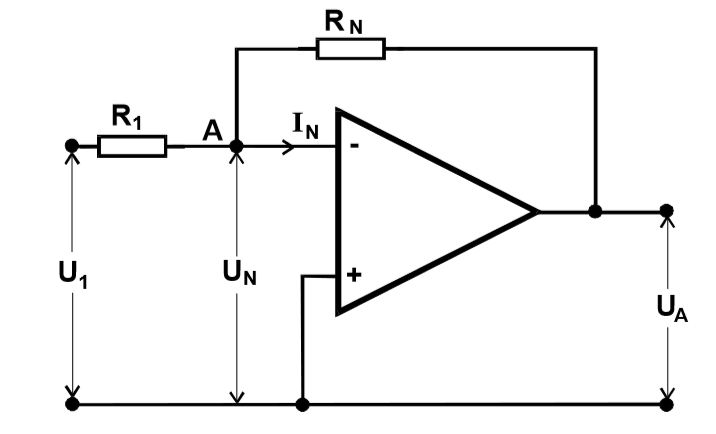
\includegraphics[width=\textwidth]{img/linear.png}
	\caption{Schaltbild eines Operationsverstärkers}
	\label{abb:linear}
\end{figure}

Die Verstärkung des Linearverstärkers hat somit die Form
\begin{equation}
V^\prime = - \frac{R_N}{R_1}
\end{equation}
bzw. unter Berücksichtigung der Eigenschaften eines realen Operationsverstärkers
\begin{equation}
\frac{1}{V^\prime} = - \frac{U_1}{U_A} = \frac{1}{V} + \frac{R_1}{R_N} \left( 1 + \frac{1}{V} \right) \approx \frac{1}{V} + \frac{R_1}{R_N}.
\label{effVerstaerkung}
\end{equation}


\subsubsection{Elektrometerverst{\"a}rker}
Bei Messungen mit hochohmigen Spannungsquellen ist es möglich, das der geringe Eingangswiderstand des Linearverstärkers die Messung Verfäschen. Die
Elektrometerverstärkerschaltung gem. \ref{abb:elektro} besitzt diesen Nachteil nicht, da die Eingangsspannung direkt am invertierenden Eingang des Operationsverstärkers anliegt, was für einen hohen Eingangswiderstand
sorgt.
\begin{figure}
 	\centering
 	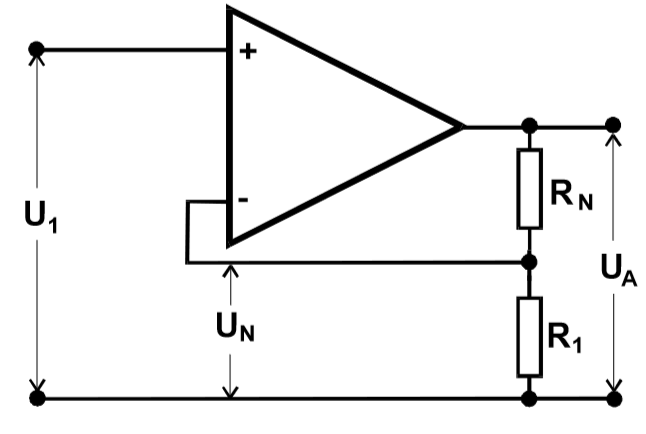
\includegraphics[width=\textwidth]{img/elec.png}
 	\caption{Schaltbild eines Operationsverstärkers}
 	\label{abb:elektro}
\end{figure}
Hier berechet sich der Verstärkungsfaktor gem.:
\begin{equation}
V' = \frac{U_A}{U_1}=\frac{R_N + R_1}{R_1}.
\end{equation}


\subsubsection{Amperemeter}
Zur Messung von kleinen Strömen wird ein klener Eingangswiderstand benötigt. Dazu kann ein Amperemeter gem \ref{} verwendet werden, bei dem doie Ausgangsspannung proportional zum Eingangsstrom ist:
\begin{equation}
U_A = IR_N.
\end{equation}
\begin{figure}
 	\centering
 	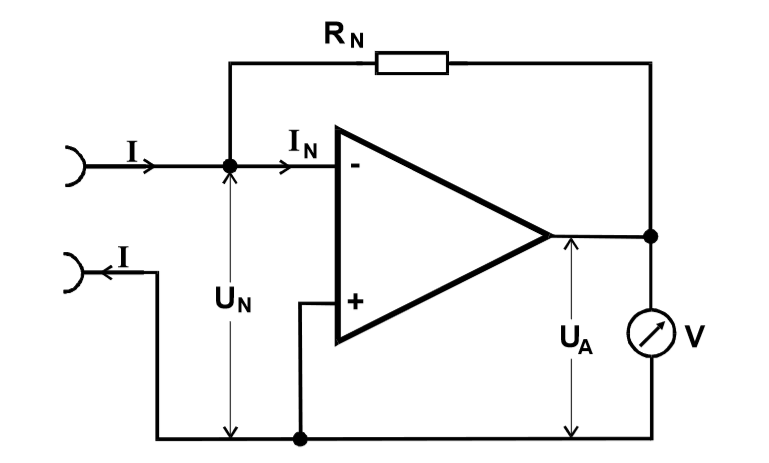
\includegraphics[width=\textwidth]{img/ampere.png}
 	\caption{Schaltbild eines Operationsverstärkers}
 	\label{abb:ampere}
\end{figure}
Der Eingangswiderstand der Schaltung ist
\begin{equation}
r_e = \frac{R_N}{V}
\end{equation}

\subsubsection{Integrator und Differentiator}
Mit der in \ref{abb:int} dargestellten Schaltung wird die Eingangsspannung integiert:
\begin{figure}
 	\centering
 	\includegraphics[width=\textwidth]{int/op.png}
 	\caption{Schaltbild eines Operationsverstärkers}
 	\label{abb:int}
\end{figure}
\begin{equation}
U_A = - \frac{1}{RC} \int U_1(t)dt
\end{equation}
Beschreibt $U_1$ eine Sinusspannung $U_1 = U_0 sin(\omega t)$, so ist die Amplitude antiproportional zur Frequenz
\begin{equation}
U_A = \frac{U_0}{\omega RC} \cos(\omega t)
\end{equation}

Das Gegenstück zum Integrator ist der Differentiator. Dieser wird gem \ref{abb:diff} aufgebaut.
\begin{equation}
U_A = -RC \frac{\text{d} U_1}{\text{d} t}
\end{equation}
Für den Fall, dass das Eingangssignal wieder als Sinusspannung vorliegt ergibt sich:
\begin{equation}
U_A = -\omega RCU_0 \cos(\omega t)
\end{equation}
Somit ist die Amplitude der Ausgangsspannung proportional zur Frequenz

\begin{figure}
 	\centering
 	\includegraphics[width=\textwidth]{img/.png}
 	\caption{Schaltbild eines Operationsverstärkers}
 	\label{abb:diff}
\end{figure}


\subsubsection{Schmitt-Trigger}
Der Schmitt-Trigger wird gem. \ref{abb:sch} verschaltet. Hier liegt ein Teil der Ausgangsspannung wieder am  nicht-invertierten Eingang an. Dadurch steigt die Ausgangsspannung immer weiter an. Die Schaltung bekommt somit ein instabiles Verhalten. Der Schmitt-Triger hat nur zwei Zusände, in denen seine Ausgangsspannung $U_B$ beträgt, wenn die Eingangsspannung $\frac{R_1}{R_P} U_B$ überschreitet oder
$-U_B$ wenn die Eingangsspannung $-\frac{R_1}{R_P} U_B$ unterschreitet. Der Schmitt-Trigger ist daher ein nützliches Element für binäre Logik und Signalgeneratoren.

\begin{figure}
 	\centering
 	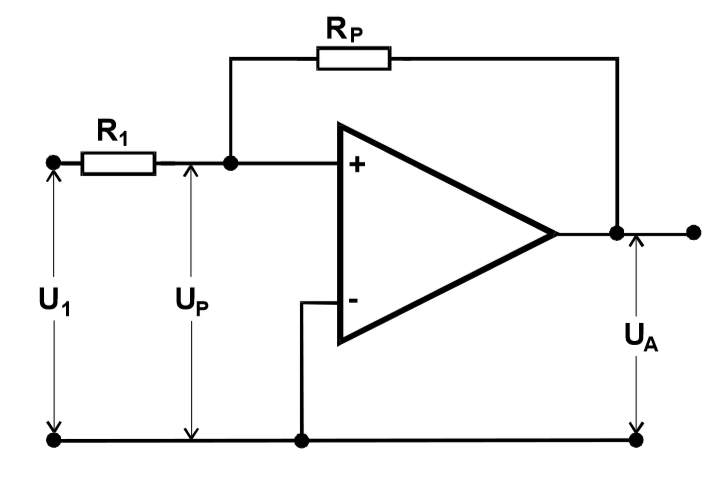
\includegraphics[width=\textwidth]{img/schmitt.png}
 	\caption{Schaltbild eines Operationsverstärkers}
 	\label{abb:sch}
\end{figure}

\subsubsection{Signalgenerator}
In \ref{abb:sig} ist der Aufbau eines Signalgenerators gezeigt. Dieser besteht aus einem Schmitt-Trigger und einem Integrator. Der Integrator integriert die durch den Schmitt-Trigger erzeugen Rechteck-Spannungen, was zu einem Dreieck-Signal führt, wobei der Ausgang des Integrators gleichzeitig der Eingang des Schmitt-Triggers ist, sodass dieser regelmäßig an der Spitze des Dreieck-Signals den Zustand ändert.

Die Integration erfolgt folgendermaßen:
\begin{equation}
U_A = - \frac{1}{RC} \int_{0}^{\frac{T}{2}} U_E(t^\prime)dt^\prime = -\frac{1}{RC} U_B \frac{T}{2}
\end{equation}
Da diese Spannung der Differenz zwischen den beiden Schwellenwerten des Schmitt-Triggers entspricht, ist
\begin{equation}
U_A = 2U_B\frac{R_1}{R_P}
\end{equation}
Diese beiden Gleichung ergeben mit der Periodendauer $T$ und der Frequenz $f$:
\begin{equation}
f = \frac{R_P}{4RCR_1}
\end{equation}

\begin{figure}
 	\centering
 	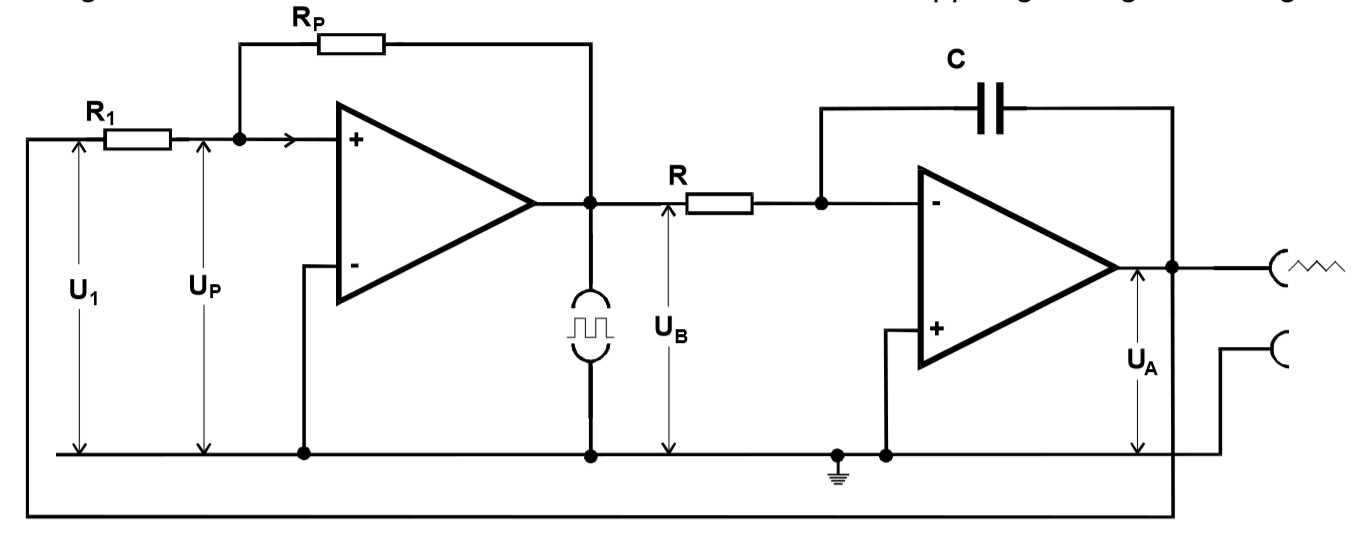
\includegraphics[width=\textwidth]{img/gen.png}
 	\caption{Schaltbild eines Operationsverstärkers}
 	\label{abb:sig}
\end{figure}

\subsubsection{Erzeugung von ged{\"a}mpften Sinusschwingungen}
Es wird ein Generator verwendet, der eine Sinusschwingung erzeugt, die mit einer abfallenden Exponentialfunktion überlagert ist. Die Schaltung ist in \ref{abb:sig2} dargestellt.

Die Schaltung besitzt die Differentialgleichung
\begin{equation}
\frac{\text{d}^2 U_A}{\text{d}t^2} - \frac{\nu}{10RC} \frac{\text{d} U_A}{\text{d}t} + \frac{1}{R^2 C^2} U_A = 0
\end{equation}
mit der Lösung
\begin{equation}
U_A(t) = U_0 \exp(\frac{\nu t}{20 RC}) \sin(\frac{t}{RC})
\end{equation}
Mit der Schwingungsdauer
\begin{equation}
T = 2\pi RC
\end{equation}
und der Abklingdauer
\begin{equation}
\tau = \frac{20 RC}{\nu}.
\end{equation}

\begin{figure}
 	\centering
 	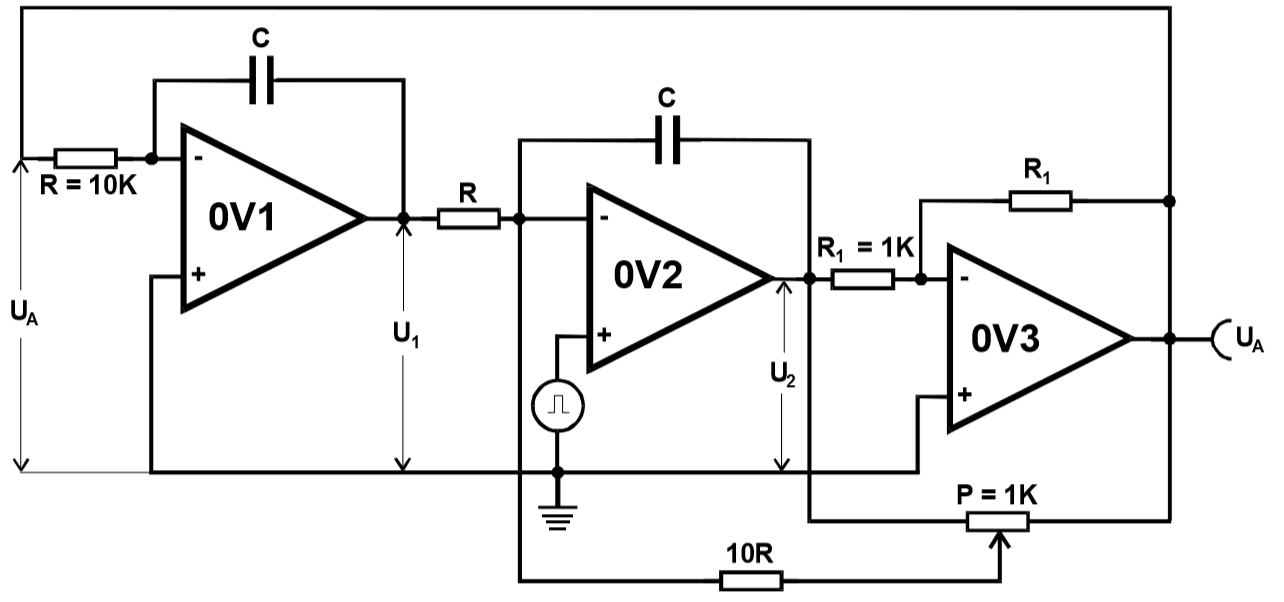
\includegraphics[width=\textwidth]{img/sin.png}
 	\caption{Schaltbild eines Operationsverstärkers}
 	\label{abb:sig2}
\end{figure}

\section{Durchf{\"u}hrung}
Zuerst wird eine Schaltung gem. \ref{abb:linear} aufgebaut und für vier verschiedene Verstärkungen (einstellbar über den Widerstand in der Gegenkopplung)
die Frequenz über mehrere Größenordnungen variert. Es ist eine frequenzabhängige Abnahme der Verstärkung zu beobachten.

Als nächstes wird ein Umkehrintegrator gem. \ref{abb:int} aufgebaut, sodass die 
Frequenzabhängigkeit der Amplitude des Ausgangssignals untersucht werden kann. Es 
ist darauf zu achten, dass der Frequenzbereich so gewählt wird, das der Umkehrintegrator
auch als solcher arbeitet.

Dieses Vorgehen wiederholt man für den Differentiator gem. \ref{abb:diff}.

Als nächste Schaltung wird der Schmitt-Triger gem. \ref{abb:schmitt} untersucht.
An den Eingang des Schmitt-Triggers wird ein Funktionsgenrator angeschlosssen und an den Ausgang 
ein Oszilloskop. Die Amplitude des Eingangssignals wird von null ausgehend solange erhöht,
bis die Schaltung anfängt zu kippen. Daraufhin wird der Scheitelwert dieser Spannung sowie  
sie Größe $2U_B$ gemessen.

Für den Dreiecksgenerator gem. \ref{abb.sig} wird die Zeitabhängigkeit der Ausgangspannung mit einem
Oszilloskop kontrolliert sowie die Frequenz und die Amplitude des erzeugten Signals gemessen.

Abschließend wird ein Signalgenerator gem. \ref{abb.sig2} aufgebaut. An den Ausgang der Schaltung
wird ein Oszilloskop angeschlossen. Über das Potentiometer ist es möglich die Dämpfung der Schwingungs
einzustellen. Das Potentiometer wird so eingestellt, dass das Ausgangssignal ungedämpft ist. Von diesem Signal wird
die Frequenz bestimmt. Daraufhin wird die Dämpfung auf ein Maximum erhöht und 
die Schwingung mit einem Dreieck-Signal angeregt, wobei die Periodendauer des Eingangssignals groß ist
gegenüber der Abklingdauer der gedämpften Schwingung. Von dem Ausgangssignal wird ein Bild erstellt.